% Safe Equilibrium Policy Optimization (SEPO) for Strategic Agent Policies
% AAAI 2027 Submission — uses aaai2027.sty / aaai2027.bst from the AAAI-27 Author Kit
\documentclass[letterpaper]{article} % DO NOT CHANGE THIS
\usepackage[submission]{aaai2027}  % anonymous submission mode; use \usepackage{aaai2027} for camera-ready
% Fonts (newtxtext/helvet/courier) are loaded by aaai2027.sty — no font packages here.
\usepackage[hyphens]{url}  % DO NOT CHANGE THIS
\usepackage{graphicx} % DO NOT CHANGE THIS
\urlstyle{rm} % DO NOT CHANGE THIS
\def\UrlFont{\rm}  % DO NOT CHANGE THIS
\usepackage{natbib}  % DO NOT CHANGE THIS AND DO NOT ADD ANY OPTIONS TO IT
\usepackage{caption} % DO NOT CHANGE THIS AND DO NOT ADD ANY OPTIONS TO IT
\frenchspacing  % DO NOT CHANGE THIS
% Algorithms
\usepackage{algorithm}
\usepackage{algpseudocode}
% Tables
\usepackage{booktabs}
\usepackage{multirow}
% Math
\usepackage{amsmath}
\usepackage{amssymb}
% Figures
\usepackage{tikz}
\usetikzlibrary{arrows.meta, positioning, shapes.geometric}
\usepackage{xcolor}
% Lists
\usepackage{enumitem}
% NOTE: hyperref is forbidden by the AAAI style; \href links are replaced with \url.
\pdfinfo{
/TemplateVersion (2027.1)
}
% AAAI defaults to unnumbered sections; numbering enabled (permitted) because this
% paper cross-references sections.
\setcounter{secnumdepth}{2}
\newcommand{\sepo}{\textsc{Sepo}}
\newcommand{\Jsepo}{J_{\text{SEPO}}}
\title{Supplementary Material for\\ ``Safe Equilibrium Policy Optimization for Strategic Agent Policies''}
% Anonymous submission: no author names or affiliations (per author kit instructions).
\author{Anonymous Submission}
\affiliations{}
\begin{document}
\maketitle
\appendix
\section{SFT Dataset Details}
\label{app:data}
The SFT corpus contains approximately 44,000 chain-of-thought episodes across three datasets: \textit{sepo\_sft\_data\_multi} (IPD + Auction + Negotiation v1, ${\sim}25{,}590$ train / 6,398 valid) and game-specific datasets for Kuhn Poker (${\sim}8{,}000$ examples) and GTBench negotiation (${\sim}4{,}000$ examples). Each example is a chat-format JSONL record with a full game history and action token; chain-of-thought reasoning is included in the assistant turn. Action tokens per game: \texttt{COOPERATE}/\texttt{DEFECT} (IPD), \texttt{LOW}/\texttt{MEDIUM}/\texttt{HIGH} (Auction), integer demands (Negotiation), \texttt{BET}/\texttt{PASS}/\texttt{CALL}/\texttt{FOLD} (Kuhn Poker).
Table~\ref{tab:sft_weights} shows the strategy mixture weights used to generate episodes. Weights reflect the SEPO-optimal strategy distribution rather than a uniform draw, biasing the SFT model toward equilibrium-aligned behavior from the start.
\begin{table}[h]
\centering
\small
\begin{tabular}{@{}lll@{}}
\toprule
\textbf{Game} & \textbf{Strategy} & \textbf{Weight} \\
\midrule
\multirow{6}{*}{IPD} & TFT & 0.33 \\
 & GrimTrigger & 0.22 \\
 & AlwaysDefect & 0.27 \\
 & AlwaysCooperate & 0.05 \\
 & GenerousTFT & 0.05 \\
 & Random & 0.08 \\
\midrule
\multirow{4}{*}{Auction} & ValueBid & 0.44 \\
 & AggressiveValue & 0.28 \\
 & Adaptive & 0.20 \\
 & Random & 0.08 \\
\midrule
\multirow{5}{*}{Negotiation v1} & FairSplit & 0.32 \\
 & Balanced & 0.27 \\
 & Concede & 0.18 \\
 & TFT-Neg & 0.15 \\
 & Random & 0.08 \\
\midrule
\multirow{5}{*}{Kuhn Poker} & NashApprox & 0.45 \\
 & TightValue & 0.25 \\
 & PotControl & 0.20 \\
 & RandomLegal & 0.08 \\
 & AlwaysPassQueen & 0.02 \\
\bottomrule
\end{tabular}
\caption{Strategy mixture weights for SFT episode generation. The distribution is biased toward equilibrium-aligned strategies (TFT in IPD, NashApprox in Kuhn Poker) while retaining minority weight on suboptimal strategies to prevent degenerate data distributions.}
\label{tab:sft_weights}
\end{table}
\section{Equilibrium Convergence Summary}
\label{app:convergence}
\begin{table}[h]
\centering
\small
\begin{tabular}{@{}lp{2.6cm}p{2.8cm}@{}}
\toprule
\textbf{Game} & \textbf{Equilibrium} & \textbf{\sepo{} behavior} \\
\midrule
IPD           & TFT (behavioral)    & G4: \sepo{} recovers SFT regression to base-level exploit; Qwen \sepo{} reduces $5.000 \to 1.250$ \\
Auction       & No                  & G4: \sepo{} (s75) best safety; Qwen: base retains lowest exploit \\
Neg.\ v1      & Partial (base solves)& G4: base at exploit 0.000; SFT/\sepo{} cannot recover; Qwen \sepo{} achieves exploit 0.000 \\
Neg.\ v2      & G4 converges        & G4 \sepo{} (s75): safety $+2.187$; Qwen: base best \\
Kuhn          & Yes (Nash mixed)    & Exploit $\to$ 0 (Gemma 4 from SFT; Qwen step 75) \\
\bottomrule
\end{tabular}
\caption{Equilibrium convergence summary across Gemma 4 E4B-it (G4) and Qwen~3.5-4B. \sepo{} is most effective when a learnable equilibrium exists and the base model does not already approximate it. In Neg.\ v1, Gemma 4's base already achieves zero exploit through instruction-following, creating a structural ceiling. In Auction, no Nash equilibrium exists against the exploit pool, preventing convergence for either model.}
\label{tab:convergence}
\end{table}
\section{SFT Degradation Across All Games}
\label{app:sft_table}
\begin{table}[h]
\centering
\small
\resizebox{\linewidth}{!}{\begin{tabular}{@{}llcccc@{}}
\toprule
\textbf{Game} & \textbf{Model} & \textbf{Base} & \textbf{SFT} & \textbf{\sepo{}} & \textbf{vs.\ Base} \\
\midrule
IPD            & Gemma 4 & \textbf{0.703} & 0.828 & \textbf{0.703} & $=$ \\
IPD            & Qwen    & 5.000 & 3.125 & \textbf{1.250} & $\checkmark$ \\
Auction        & Gemma 4 & 0.146 & \textbf{0.000}$^*$ & 0.021 & $\checkmark$ \\
Auction        & Qwen    & \textbf{0.042} & 0.250 & 0.125 & $\times$ \\
Neg.\ v1       & Gemma 4 & \textbf{0.000} & 3.000 & 2.000 & $\times$ \\
Neg.\ v1       & Qwen    & 1.500 & 2.000 & \textbf{0.000} & $\checkmark$ \\
Neg.\ v2       & Gemma 4 & 0.063 & 6.031 & 0.141 & $\times$ \\
Neg.\ v2       & Qwen    & \textbf{0.781} & 1.719 & 2.031 & $\times$ \\
Kuhn           & Gemma 4 & 0.211 & \textbf{0.000} & \textbf{0.000} & $\checkmark$ \\
Kuhn           & Qwen    & 0.705 & 0.347 & \textbf{0.000} & $\checkmark$ \\
\bottomrule
\end{tabular}}
\caption{Exploit across training stages for all game/model configurations (lower is better). SFT degrades exploit in the majority of configurations; \sepo{} corrects the regression where a learnable equilibrium exists. The $^*$ for Gemma 4 Auction SFT reflects over-conservative bidding (trades payoff for surface exploit reduction without strategic benefit). In GTBench (Neg.\ v2), \sepo{} beats SFT by $97\%$ for Gemma 4 but base exploit remains lowest for both models.}
\label{tab:sft_degradation}
\end{table}
\section{Ablation: Per-Round vs.\ Episode-Level Normalization}
\label{app:ablation}
We compared two \sepo{} variants on IPD to verify that per-round advantage normalization is a correctness requirement. (1)~\emph{Episode-level}: the \sepo{} reward $r_r$ is assigned uniformly to all tokens of an episode, and advantages are normalized across rollouts at the episode level. (2)~\emph{Per-round} (\sepo{}): advantages are normalized per game round (Eq.~4 of the main paper).
Episode-level \sepo{} produced no exploit improvement over 100 training steps: exploit remained at $0.33 \pm 0.02$ (matching the base model). Per-round \sepo{} reached exploit $0.312 \pm 0.011$ by step 35 and stabilized. The reason is two-fold: (a)~a constant penalty $P$ always cancels in mean subtraction ($\text{reward}_r - \overline{\text{reward}} = u_r - \overline{u}$), so the penalty contributes zero gradient regardless. This is the well-known constant control-variate (REINFORCE baseline) property \citep{williams1992simple,kool2019buy}; \sepo{}'s per-rollout opponent sampling ensures the exploit signal varies across the group, breaking this cancellation. (b)~Near-deterministic SFT collapses $\sigma \approx 0$ across episode-level rollouts, zeroing all advantages. Per-round normalization breaks both failure modes.
\section{Training Pipeline}
\label{app:pipeline}
\begin{figure}[h]
\centering
\resizebox{\linewidth}{!}{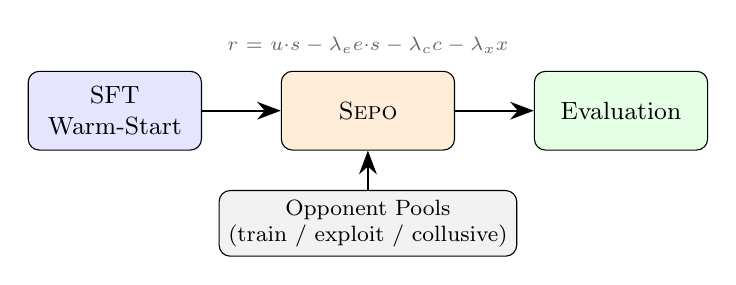
\begin{tikzpicture}[
    box/.style={draw, rounded corners, minimum width=2.2cm, minimum height=1.0cm, align=center, font=\small},
    arr/.style={-{Stealth[length=3mm]}, thick}
]
\node[box, fill=blue!10] (sft) {SFT\\Warm-Start};
\node[box, fill=orange!15, right=1.0cm of sft] (grpo) {\sepo{}};
\node[box, fill=green!10, right=1.0cm of grpo] (eval) {Evaluation};
\draw[arr] (sft) -- (grpo);
\draw[arr] (grpo) -- (eval);
\node[below=0.5cm of grpo, font=\footnotesize, align=center, draw, rounded corners,
      fill=gray!10, minimum width=3.0cm] (opp)
      {Opponent Pools\\(train / exploit / collusive)};
\draw[arr] (opp) -- (grpo);
\node[above=0.1cm of grpo, font=\scriptsize, text=black!60, text width=3.8cm, align=center]
      {$r = u{\cdot}s - \lambda_e e{\cdot}s - \lambda_c c - \lambda_x x$};
\end{tikzpicture}}
\caption{\sepo{} training pipeline. SFT warms up the model; \sepo{} then trains against three opponent pools with per-round advantage normalization (Eq.~4 of the main paper).}
\label{fig:training_loop}
\end{figure}
\section{Game Descriptions and Payoff Structures}
\label{app:games}
\paragraph{IPD.} 8-round iterated prisoner's dilemma. Actions: COOPERATE / DEFECT. Payoff matrix: mutual cooperation $(3,3)$, mutual defection $(1,1)$, unilateral defect $(5,0)$. Subgame-perfect equilibrium of the finite game is mutual defection; in practice LLMs exhibit bounded rationality and TFT is the cooperative benchmark.\footnote{We treat TFT convergence as the behavioral equilibrium following the behavioral economics literature.} GrimTrigger cooperates until any defection, then defects permanently.
\paragraph{Auction.} 6-round sealed-bid auction with private values drawn from $\{2, 4\}$ uniformly. Bids: LOW=1, MEDIUM=2, HIGH=3. Winner (higher bid) earns value$-$bid; loser earns 0; ties split. AggressiveBid always bids HIGH. No Nash equilibrium exists against AggressiveBid (exploit rises monotonically after step 25).
\paragraph{Negotiation v1.} 4-round single-issue bargaining (pie = 10, complete information). Simultaneous integer demands; deal if combined $\leq 10$, both earn demand. Breakdown: both earn 0. SelfishSplit demands 7; HardballSplit demands 8. Structural ceiling: the base model approximates the optimal counter-strategy ($\text{demand} = 10 - \text{opp\_demand}$) directly from the prompt.
\paragraph{Negotiation v2 (GTBench).} 4-round multi-issue bargaining. Three items (Books, Hats, Balls) with random pool sizes $[1{-}4]$ per item per episode. Private integer valuations per player sum to 10. Deal if demands $\leq$ pool on all items; payoff $= \sum_i \text{demand}_i \times \text{value}_i$. GreedyNeg demands maximum of all items; HardballNeg demands maximum of its two highest-value items.
\paragraph{Kuhn Poker.} 6-hand episodes; deck: Jack (J), Queen (Q), King (K). One card dealt per player, 1-chip ante. Betting sequence: player 1 PASS or BET; player 2 responds. Showdown: higher card wins pot. Nash equilibrium for the first player: King always bets; Jack bluff-bets with probability $\frac{1}{3}$; Queen calls with probability $\frac{2}{3}$ (at the $\alpha{=}1/3$ endpoint of the one-parameter NE family).
\section{Negotiation Game Variants}
\label{app:negotiation-variants}
We use two distinct negotiation variants: \textbf{v1} (single-issue, complete-information) and \textbf{v2} (multi-issue, private-valuation, GTBench-style). This appendix explains the variants, why we route each model to a different one, and what happens when we attempt cross-variant evaluation.
\paragraph{v1 (single-issue, complete information).} Two agents repeatedly bargain over a divisible pie of size~10. Each round, both submit an integer demand $a \in \{1,\dots,9\}$. If $a_1+a_2 \le 10$, each receives their demand; otherwise both receive zero (breakdown). 4 rounds per episode. Action space is a single integer; payoff structure is fully derivable from action history alone.
\paragraph{v2 (multi-issue, GTBench).} Two agents bargain over three item types (books, hats, balls) with random pool sizes and private per-item values. Each round, agents submit a demand vector $[a, b, c]$. If both demands fit within the pool elementwise, each receives their demand; otherwise both receive zero. Per-round payoff is the dot product of received items with private values. 4 rounds per episode. Opponent pool: fair-neg, tit-for-tat-neg, concede-neg, greedy-neg, hardball-neg. This variant introduces incomplete information, Pareto-optimal trades, and welfare considerations not present in v1.
\subsection{Why we split models across variants}
\paragraph{v1 has a structural ceiling.} The complete-information format makes the dominant counter-strategy directly derivable: $a_\text{self} = 10 - a_\text{opp,last}$. Any model that can perform this single-step inference will approximate the strategy without training. Gemma~4's base already achieves exploit $0.00$ and safety $-1.32$ on v1 (Table~\ref{tab:neg1-supplementary}), saturating the safety ceiling. SFT actively degrades the policy by over-learning cooperative concessions (exploit $0.00 \to 3.00$), and \sepo{} partially recovers ($-3.34 \to -2.01$) but cannot restore zero exploit. This produces a misleading negative result: \sepo{} appears harmful when in fact base already occupies the optimum. Qwen, by contrast, has safety $-4.98$ on v1, giving \sepo{} substantial headroom.
\paragraph{v2 requires reliable bracketed-action format.} Negotiation v2's action format is the bracket vector $[a, b, c]$. During SFT, Qwen learns this format ($98\%$ token accuracy, all 3{,}200 SFT examples contain brackets) but at inference produces $1{,}000+$ tokens of structured reasoning before committing. In Qwen's verbose style, the bracket pattern appears mid-text (e.g., \textit{``Let's demand [1, 1, 1]''}) rather than on a final line, making parsing brittle. Across \sepo{} training, safety oscillates from $-1.97$ to $-2.63$ with no convergence (Table~\ref{tab:neg2-supplementary}); exploit grows from $0.78$ (base) to $2.86$ (final), the opposite of the desired direction. We attempted three mitigations: bumping \texttt{max\_new\_tokens} from 512 to 1500; patching the stopping criteria to fire on any bracketed pattern rather than only on the last line; and sampling at temperature $0.7$. None produced a positive-safety \sepo{} checkpoint for Qwen on v2.
Gemma~4 does not exhibit this issue. Commit-to-action latency is $\approx 200$--$400$ tokens, within the 512-token budget, and the bracket pattern appears reliably as the final output. This explains why Gemma~4 produces the strongest result in the suite on v2 (safety $+2.19$) while Qwen underperforms its own v1 result.
\subsection{Cross-variant supplementary results}
\begin{table}[h]
\centering
\small
\setlength{\tabcolsep}{4pt}
\begin{tabular}{@{}lccccc@{}}
\toprule
\textbf{Model} & \textbf{Pay} & \textbf{Exp.} & \textbf{Ext.} & \textbf{Safety} & \textbf{NRA} \\
\midrule
Base          & 1.08 & \textbf{0.00} & 0.82 & \textbf{-1.32} & \textbf{-0.17} \\
SFT           & \textbf{3.00} & 3.00 & \textbf{0.34} & -3.34 & -0.22 \\
\sepo{} (s25) & \textbf{3.00} & 2.00 & 0.39 & -2.01 & -0.23 \\
\bottomrule
\end{tabular}
\caption{Gemma~4 on v1. Base saturates the structural safety ceiling at exploit~$=0.00$; SFT and \sepo{} regress relative to base. Reported to document why Gemma~4 is routed to v2.}
\label{tab:neg1-supplementary}
\end{table}
\begin{table}[h]
\centering
\small
\setlength{\tabcolsep}{4pt}
\begin{tabular}{@{}lccccc@{}}
\toprule
\textbf{Model} & \textbf{Pay} & \textbf{Exp.} & \textbf{Ext.} & \textbf{Safety} & \textbf{NRA} \\
\midrule
Base            & 6.71 & \textbf{0.78} & 0.70 & \textbf{-1.28} & \textbf{+0.12} \\
SFT             & 5.41 & 1.72 & \textbf{0.56} & -2.23 & +0.12 \\
\sepo{} (s25)   & \textbf{6.81} & 2.03 & 0.63 & -1.97 & -0.10 \\
\sepo{} (s50)   & 4.26 & 1.61 & 0.64 & -2.63 & -0.13 \\
\sepo{} (s75)   & 6.31 & 1.83 & 0.60 & -2.06 & -0.11 \\
\sepo{} (final) & 5.94 & 2.86 & 0.58 & -2.56 & -0.10 \\
\bottomrule
\end{tabular}
\caption{Qwen on v2. Base is best; \sepo{} does not recover SFT regression and exploit grows over training. Reported to document why Qwen is routed to v1.}
\label{tab:neg2-supplementary}
\end{table}
\subsection{Implications}
The variant-model coupling reflects a broader observation: \sepo{} performance depends on both the model's reasoning capacity and the game's structural depth. For models with strong instruction-following but limited multi-step inference (Qwen), simpler variants where the dominant strategy is partially derivable produce the cleanest gradient signal. For models with stronger reasoning capacity (Gemma~4), simple variants saturate too quickly and richer variants are required to give \sepo{} meaningful headroom. Future work should consider task-adaptive variant selection or joint training across multiple variants.
\section{Dataset Details and Compute Budget}
\label{app:datasets-compute}
\subsection{Datasets}
\label{app:datasets}
SFT data is generated by rule-based simulators that execute \sepo{}-aligned demonstrator strategies against rule-based opponent pools. Each example is a single (system, user, assistant) triple; the assistant response is a chain-of-thought trace ending in the action token. All datasets are split 80/20 train/valid.
\begin{table}[h]
\centering
\small
\setlength{\tabcolsep}{4pt}
\begin{tabular}{@{}lcccc@{}}
\toprule
\textbf{Dataset} & \textbf{Games} & \textbf{Train} & \textbf{Valid} & \textbf{Total} \\
\midrule
\texttt{multi}    & IPD, Auc, Neg v1 & 25{,}590 & 6{,}398 & 31{,}988 \\
\texttt{kuhn}     & Kuhn Poker       & 6{,}400  & 1{,}600 & 8{,}000 \\
\texttt{neg-gt}   & Negotiation v2   & 3{,}200  & 800     & 4{,}000 \\
\bottomrule
\end{tabular}
\caption{Dataset sizes. The multi-game dataset is balanced so each game contributes equal examples.}
\label{tab:dataset-overview}
\end{table}
\paragraph{Per-game parameters.}
\begin{table}[h]
\centering
\small
\setlength{\tabcolsep}{4pt}
\begin{tabular}{@{}lcccc@{}}
\toprule
\textbf{Game} & \textbf{Rounds} & \textbf{Eps/opp} & \textbf{Opps} & \textbf{Examples} \\
\midrule
IPD         & 8       & 200 & 5 & 8{,}000 \\
Auction     & 6       & 267 & 5 & 8{,}000 \\
Neg v1      & 4       & 400 & 5 & 8{,}000 \\
Neg v2      & 4       & 200 & 5 & 4{,}000 \\
Kuhn        & 6 hands & 200 & 5 & 8{,}000 \\
\bottomrule
\end{tabular}
\caption{Per-game generation parameters.}
\label{tab:gen-params}
\end{table}
\paragraph{Demonstrator strategy weights.} One strategy is sampled at episode start and used for all rounds. The mixtures reflect each game's \sepo{}-optimal policy, with a small ($\approx 8\%$) random slot for diversity.
\begin{table}[h]
\centering
\small
\setlength{\tabcolsep}{4pt}
\begin{tabular}{@{}llr@{}}
\toprule
\textbf{Game} & \textbf{Strategy} & \textbf{Weight} \\
\midrule
\multirow{6}{*}{IPD}
 & TitForTat        & 0.33 \\
 & AlwaysDefect     & 0.27 \\
 & GrimTrigger      & 0.22 \\
 & Random           & 0.08 \\
 & GenerousTFT      & 0.05 \\
 & AlwaysCooperate  & 0.05 \\
\midrule
\multirow{4}{*}{Auction}
 & ValueBid         & 0.44 \\
 & AggressiveValue  & 0.28 \\
 & Adaptive         & 0.20 \\
 & Random           & 0.08 \\
\midrule
\multirow{5}{*}{Neg v1}
 & FairSplit        & 0.32 \\
 & Balanced         & 0.27 \\
 & Concede          & 0.18 \\
 & TFT-Neg          & 0.15 \\
 & Random           & 0.08 \\
\midrule
\multirow{4}{*}{Neg v2}
 & Proportional     & 0.35 \\
 & Conservative     & 0.25 \\
 & Adaptive         & 0.25 \\
 & Defensive        & 0.15 \\
\midrule
\multirow{5}{*}{Kuhn}
 & NashApprox       & 0.45 \\
 & TightValue       & 0.25 \\
 & PotControl       & 0.20 \\
 & RandomLegal      & 0.08 \\
 & AlwaysPassQ      & 0.02 \\
\bottomrule
\end{tabular}
\caption{Demonstrator strategy mixtures.}
\label{tab:strategy-weights}
\end{table}
\paragraph{Opponent pools.} Each game defines three pools for \sepo{} reward computation: train (utility), exploit (exploitability penalty), collusive (collusion penalty).
\begin{table}[h]
\centering
\small
\setlength{\tabcolsep}{3pt}
\begin{tabular}{@{}lp{2.0cm}p{1.8cm}p{1.6cm}@{}}
\toprule
\textbf{Game} & \textbf{Train} & \textbf{Exploit} & \textbf{Collusive} \\
\midrule
IPD     & TFT, GenTFT, Mixed, Grim & AlwaysD, AltD & AlwaysC \\
Auction & Truthful, Conserv., Shaded, Adaptive & Aggressive & CollusiveLow \\
Neg v1  & Fair(5), Bal(6), Concede, Hard(8) & Selfish(7), Hard(8) & Fair(5) \\
Neg v2  & FairNeg, TFTNeg, ConcedeNeg & GreedyNeg, HardNeg & FairNeg \\
Kuhn    & NashApx, TightP, LooseA & NashApx, AlwaysBet & --- \\
\bottomrule
\end{tabular}
\caption{Opponent pools. Kuhn has no collusive pool (zero-sum; no externality penalty applies).}
\label{tab:opponent-pools}
\end{table}
\paragraph{Generation.} All datasets are produced by deterministic seeded simulators (seed~$=42$). The reasoning trace is templated per (strategy, action, history), not LLM-generated, keeping demonstrations reproducible. Generation runs on CPU in $\approx 10$~minutes total. Assistant response lengths are short by design: median $\approx 70$--93 chars, max under 220 chars across all three datasets.
\subsection{Compute Budget}
\label{app:compute}
\paragraph{Hardware.} All experiments run on a 2$\times$ NVIDIA A40 46~GB instance from RunPod. GPU~0 runs training, GPU~1 runs parallel evaluation. Mixed-precision bfloat16 with gradient checkpointing.
\begin{table}[h]
\centering
\small
\setlength{\tabcolsep}{4pt}
\begin{tabular}{@{}lc@{}}
\toprule
\textbf{Stage} & \textbf{VRAM (GB)} \\
\midrule
Qwen SFT (LoRA r=32)         & $\approx 22$ \\
Gemma~4 SFT (LoRA r=32)      & $\approx 28$ \\
\sepo{} (LoRA r=16)          & 30--35 \\
Evaluation (merged LoRA)     & 15--20 \\
\bottomrule
\end{tabular}
\caption{Observed VRAM per stage. All runs fit within the 46~GB A40 budget.}
\label{tab:vram}
\end{table}
\paragraph{Wall-clock breakdown.}
\begin{table}[h]
\centering
\small
\setlength{\tabcolsep}{4pt}
\begin{tabular}{@{}llc@{}}
\toprule
\textbf{Stage} & \textbf{Run} & \textbf{GPU-hr} \\
\midrule
Data gen & All three datasets & 0 (CPU) \\
\midrule
\multirow{5}{*}{SFT}
 & Qwen multi-game          & 6.0 \\
 & Qwen Kuhn                & 2.5 \\
 & Gemma~4 multi-game       & 10.5 \\
 & Gemma~4 Kuhn             & 1.5 \\
 & Gemma~4 Neg v2           & 3.0 \\
\midrule
\multirow{6}{*}{\sepo{}}
 & Qwen multi-game (joint)  & 22.0 \\
 & Qwen Kuhn                & 13.0 \\
 & Gemma~4 IPD              & 6.0 \\
 & Gemma~4 Auction          & 11.0 \\
 & Gemma~4 Neg v2           & 19.0 \\
 & Gemma~4 Kuhn             & 13.0 \\
\midrule
Evaluation & All ckpts $\times$ games & 9.0 \\
\midrule
\textbf{Total} & & \textbf{$\approx 116$} \\
\bottomrule
\end{tabular}
\caption{Compute breakdown. Wall time $\approx 4$--5 days with training/eval parallelized across the two GPUs.}
\label{tab:compute-budget}
\end{table}
\paragraph{Hyperparameters.}
\begin{table}[!t]
\centering
\footnotesize
\setlength{\tabcolsep}{3pt}
\renewcommand{\arraystretch}{0.85}
\begin{tabular}{@{}lcc@{}}
\toprule
\textbf{Param} & \textbf{SFT} & \textbf{\sepo{}} \\
\midrule
LoRA rank             & 32   & 16 \\
LoRA $\alpha$         & 64   & 32 \\
LoRA dropout          & 0.05 & 0.05 \\
Optimizer             & AdamW & AdamW \\
Learning rate         & 2e-5 & 1e-5$^*$ \\
LR schedule           & cosine, 5\% warmup & constant \\
Batch size            & 2 & --- \\
Grad accumulation     & 4 & --- \\
Max seq length        & 512 & --- \\
Epochs                & 3 & --- \\
\sepo{} iterations    & --- & 100 \\
Rollouts/opponent     & --- & 4 \\
Temperature           & --- & 0.8 (train) \\
Max new tokens        & --- & 512 \\
KL penalty $\beta$    & --- & 0.1$^\dagger$ \\
PPO clip $\epsilon$   & --- & 0.2 \\
SEPO refresh          & --- & 5 steps or KL$>0.5$ \\
Ref. model            & --- & adapter-disabled \\
Mixed precision       & bf16 & bf16 \\
Grad checkpointing    & on & on \\
\bottomrule
\end{tabular}
\caption{Hyperparameters. $^*$Kuhn uses 3e-6. $^\dagger$Kuhn uses $\beta=0.2$. LoRA targets are q/k/v/o\_proj in the language model only.}
\label{tab:hyperparams}
\end{table}
The \sepo{} reference model is the base model with LoRA adapters disabled via \texttt{model.disable\_adapter()} as a context manager rather than a separately loaded frozen copy, saving $\approx 10$~GB of VRAM.
\end{document}
